\section{Implementation}
\label{sec:implementation}

Based on the design defined in \cref{sec:design}, we set up the infrastructure that our pipeline will interact with, using Docker Compose first.
Then, the pipeline itself will be implemented to ingest data, transform it, and output graphs for visualization.
The pipeline's Dockerfile is shown to improve \ac{dx} next, and the resource definitions that enable a production deployment to Kubernetes are provided in the final subsection.

\subsection{Infrastructure}
\label{sec:implementation-infrastructure}

Before implementing the custom code for the pipeline, we first set up the infrastructure components that the pipeline will interact with.
MinIO will be configured for storage and Spark for compute.

The services defined in the following subsections will use various ports.
To maintain an overview of all ports used in the upcoming service definitions, a summary is provided in \cref{sec:appendix-ports}.

\subsubsection{Storage}
\label{sec:implementation-infrastructure-storage}

For \textit{S3} storage, we use MinIO, and for compute, we use Spark with Iceberg support.
The latter is provided by Databricks as a container image.

Two options were evaluated for local multi-container runtimes for development: Kubernetes, to stay as close as possible to the production environment, and \href{https://www.docker.com/}{\textit{Docker}} Compose, due to specific challenges in the local Kubernetes setup.
The challenges faced with setting up Kubernetes locally are described in detail in \cref{sec:appendix-kubernetes}.

Kubernetes, with its advanced architecture and broad feature set, is generally more complex to set up and maintain than Docker Compose, even locally.
Therefore, setting up Kubernetes locally only makes sense if this setup effectively mirrors the production environment.
Otherwise, a simpler solution would be preferable.
In this case, mirroring the production environment involves setting up virtualized block storage with Longhorn, allowing us to test the hypothesis that data will be in reach ``quickly enough'' for efficient computation, as discussed in the storage design section \cref{sec:design-storage}.
Given the challenges referenced above, the alternative container runtime explored next is Docker Compose.

The Docker Compose setup consists mainly of a \texttt{docker-compose.yaml} file and the start/stop commands shown in \cref{lst:docker-compose-commands}\footnote{The \texttt{-d} flag moves execution to the background, freeing the console for additional commands.}.
A tool named \href{https://kompose.io/}{\textit{Kompose}} can later assist in migrating a Docker Compose definition to Kubernetes resource definitions for production deployment, so pivoting to Docker Compose does not entail a significant drawback in this case.

\begin{listing}[H]
\begin{minted}{sh}
docker-compose up (-d)
docker-compose down
\end{minted}
\caption{Docker Compose start and stop commands.}
\label{lst:docker-compose-commands}
\end{listing}

To set up storage with MinIO in Docker Compose, a storage service is defined in \cref{lst:minio-compose}.
We define a named volume, \texttt{minio\_data}, and mount it to the \texttt{/data} directory used by MinIO, ensuring that data persists across Docker Compose restarts.
Automatic restarts upon failure at the service level are desirable, as this aligns with default behaviors in cluster managers like Kubernetes or \href{https://docs.docker.com/engine/swarm/}{\textit{Docker Swarm}}\footnote{Since development sometimes requires stopping a service, such as to avoid hitting rate limits on an external server, it is appropriate to set the service's \texttt{restart} policy to \texttt{unless-stopped}.}.
We expose MinIO's S3 port, 9000, and enable MinIO's web \ac{gui} on port 9001 by modifying MinIO's default start command on line 2.
The image \texttt{minio/minio} is pulled from the \href{https://hub.docker.com/}{\textit{Docker Hub}} registry by default and is versioned with a timestamp format\footnote{A more common versioning scheme used by many other images, including those defined in sections below, is \href{https://semver.org/}{\textit{Semantic Versioning}}.}.

\begin{listing}[H]
\begin{minted}{yaml}
services:
  minio:
    command: ["server", "/data", "--console-address", ":9001"]
    environment:
      MINIO_ROOT_PASSWORD: password
      MINIO_ROOT_USER: admin
    image: minio/minio:RELEASE.2024-10-29T16-01-48Z
    ports:
      - 9000:9000
      - 9001:9001
    restart: unless-stopped
    volumes:
      - minio_data:/data
volumes:
  minio_data: {}
\end{minted}
\caption{Docker Compose definition for MinIO.}
\label{lst:minio-compose}
\end{listing}

For development, MinIO's \ac{gui} is secured by arbitrary credentials set via environment variables, which are replaced by secrets in the production environment.
It is important to note that even in development, hardcoding credentials can pose a security risk, especially in open source projects, as other users on the same network could access services on the developer's machine using the same exposed credentials.

To initialize MinIO with a bucket for storing pipeline data, we define a complementary MinIO client service as shown in \cref{lst:minio-client-compose}.
The \texttt{minio-client} service is set to start only after the \texttt{minio} service has successfully started, specified by the \texttt{depends\_on} relation.
Since the S3 protocol originated from \href{https://aws.amazon.com/}{\textit{\ac{aws}}}, the three environment variables on line 5 are standard for accessing any S3-compatible service, including MinIO in a local setup.

\begin{listing}[H]
\begin{minted}{yaml}
services:
  minio-client:
    depends_on:
      - minio
    environment:
      - AWS_ACCESS_KEY_ID=admin
      - AWS_SECRET_ACCESS_KEY=password
      - AWS_REGION=us-east-1
    entrypoint: >
      /bin/sh -c "
      until (/usr/bin/mc config host add minio http://minio:9000 admin password) do echo '...waiting...' && sleep 1; done;
      /usr/bin/mc mb minio/lakehouse;
      /usr/bin/mc anonymous set public minio/lakehouse;
      tail -f /dev/null
      "
    image: minio/mc:RELEASE.2024-10-29T15-34-59Z
    restart: unless-stopped
\end{minted}
\caption{Docker Compose definition for MinIO's client.}
\label{lst:minio-client-compose}
\end{listing}

The \texttt{entrypoint} defines a script that waits until the MinIO service is reachable via \ac{http}, then creates a bucket named \texttt{lakehouse}, makes it publicly accessible, and runs a persistent command to prevent the container from restarting.
An alternative would be to modify the \texttt{restart} property to avoid restarting on success, but we aim to stay as close as possible to typical container cluster behavior.
In Kubernetes, this service would be implemented as a \textit{Job} that restarts on failure but not on success, a feature unavailable in Docker Compose.
To work around this limitation, the final \texttt{tail -f /dev/null} command ensures the container remains running.

With the definitions for the MinIO and MinIO client services, our simple and standardized storage setup is complete.

\subsubsection{Compute}
\label{sec:implementation-infrastructure-compute}

Next, we set up Spark as the computation engine in Docker Compose.
Since Spark is intended to read from and write to Iceberg tables, Iceberg support must be added to Spark.
Additionally, it is beneficial to have a \ac{gui} during development for testing Spark commands with Iceberg support.
These requirements are fulfilled by the \texttt{spark-iceberg} container image provided by \textit{Tabular}\footnote{The backing repository was migrated to \href{https://github.com/databricks/}{Databricks' GitHub organization} during the course of this thesis.}, which we use instead of the \href{https://docs.docker.com/trusted-content/official-images/}{\textit{Docker Official Images}} \texttt{spark} image, as the latter lacks these additions.

However, the \texttt{spark-iceberg} image's latest release dates back eight months, likely due to Databricks' acquisition of the former maintaining company, Tabular~\cite{Databricks2024}.
Because Iceberg is currently under active development, using a recent Iceberg version minimizes the chance of encountering bugs.
We therefore use a custom fork of the \texttt{spark-iceberg} image, available on the \ac{ghcr}, which includes Spark \texttt{3.5.3} and Iceberg version \texttt{1.6.1}.

\begin{listing}[H]
\begin{minted}{yaml}
services:
  spark-iceberg:
    image: ghcr.io/dargmuesli/spark-iceberg:3.5.3_1.6.1
    depends_on:
      - rest
      - minio
    environment:
      - AWS_ACCESS_KEY_ID=admin
      - AWS_SECRET_ACCESS_KEY=password
      - AWS_REGION=us-east-1
    ports:
      - 7077:7077
      - 8888:8888
      - 8080:8080
      - 10000:10000
    restart: unless-stopped
    volumes:
      - ./docker/spark/entrypoint-master.sh:/opt/spark/entrypoint.sh
      - ./docker/spark/spark-defaults.conf:/opt/spark/conf/spark-defaults.conf
\end{minted}
\caption{Docker Compose definition for Spark's master.}
\label{lst:compose-spark-master}
\end{listing}

\Cref{lst:compose-spark-master} shows the Spark image running as the Spark master service.
A volume overrides Spark's default settings file, \texttt{spark-defaults.conf}, as specified on line 19, with options shown in \cref{lst:spark-defaults}, particularly to configure Spark to use a \ac{rest} catalog backed by S3 for unified storage.
The image's default entrypoint is also overridden on line 19 with a script detailed in \cref{lst:spark-master-entrypoint} that performs the following:

\begin{enumerate}
    \item Binds the Spark master to port 7077.
    \item Starts an \href{https://thrift.apache.org/}{\textit{Apache Thrift}} server on port 10000, enabling \acp{rpc} through various programming languages\footnote{The Thrift connection will be used by dbt later.}.
    \item Creates Iceberg table namespaces, notably the \texttt{default} namespace\footnote{dbt requires the \texttt{default} namespace to connect successfully.}.
\end{enumerate}

Port 8888 is used for the Spark master \ac{gui}, and port 8080 for the Jupyter Notebook \ac{gui}.
As specified on line 5, the service expects a \texttt{rest} service as a catalog interface, defined in \cref{lst:compose-rest}.

\begin{listing}[H]
\begin{minted}{yaml}
services:
  rest:
    environment:
      - AWS_ACCESS_KEY_ID=admin
      - AWS_SECRET_ACCESS_KEY=password
      - AWS_REGION=us-east-1
      - CATALOG_IO__IMPL=org.apache.iceberg.aws.s3.S3FileIO
      - CATALOG_S3_ENDPOINT=http://minio:9000
      - CATALOG_S3_PATH__STYLE__ACCESS=true
      - CATALOG_WAREHOUSE=s3://lakehouse/
    image: ghcr.io/dargmuesli/iceberg-rest:1.6.1
    ports:
      - 8181:8181
    restart: unless-stopped
\end{minted}
\caption{Docker Compose definition for Spark's \ac{rest} catalog wrapper.}
\label{lst:compose-rest}
\end{listing}

Similarly to the previously described image \texttt{spark-iceberg}, the \texttt{rest} service also uses a fork of a Tabular image called \texttt{iceberg-rest}.
It is essential to ensure that all services are configured with the same tool versions to prevent compatibility errors.
The \texttt{rest} service exposes port 8181, is configured to use MinIO as the S3 storage backend, and, importantly, is set to use S3's path-style access.

By default, the \texttt{org.apache.iceberg.aws.s3} package properties enable a \textit{Virtual Host} style for bucket access.
With Virtual Host style, buckets are accessible as subdomain-like hostnames, e.g., \texttt{http://lakehouse.minio}, where \texttt{lakehouse} is the bucket name and \texttt{minio} is the service hostname, routable in the Docker Compose default network.
In contrast, the path style makes the \texttt{lakehouse} bucket accessible at \texttt{http://minio/lakehouse}.
Docker Compose can set network aliases for services, allowing MinIO to be configured for Virtual Host-style access through the incremental configuration shown in \cref{lst:compose-mino-virtual-host}.
However, setting up Virtual Host-style access in Kubernetes is more complex due to hostname syntax limitations involving dot characters.
Therefore, the \texttt{rest} service is configured to use path-style access instead.

Finally, Spark is intended to compute in a distributed manner, requiring the addition of worker services.
Even in development, adding worker services is beneficial for verifying inter-service communication.
\Cref{lst:compose-spark-worker} shows the Docker Compose service definition for Spark workers with deployment replicas scaled to two.

\begin{listing}[H]
\begin{minted}{yaml}
services:
  spark-iceberg-worker:
    deploy:
      replicas: 2
    image: ghcr.io/dargmuesli/spark-iceberg:3.5.3_1.6.1
    depends_on:
      - spark-iceberg
    environment:
      - AWS_ACCESS_KEY_ID=admin
      - AWS_SECRET_ACCESS_KEY=password
      - AWS_REGION=us-east-1
    restart: unless-stopped
    volumes:
      - ./docker/spark/entrypoint-worker.sh:/opt/spark/entrypoint.sh
      - ./docker/spark/spark-defaults.conf:/opt/spark/conf/spark-defaults.conf
\end{minted}
\caption{Docker Compose definition for a Spark worker.}
\label{lst:compose-spark-worker}
\end{listing}

The workers use the same image as the master.
The primary distinction between the worker and the master is the entrypoint script being mounted.
The worker entrypoint script, detailed in \cref{lst:spark-worker-entrypoint}, performs the following actions:

\begin{enumerate}
    \item Installs necessary dependencies for script execution\footnote{The design of dependency installation in worker containers is evaluated in \cref{sec:evaluation-objectives}.}.
    \item Binds the worker to port 8787 and configures it to connect to the Spark master.
\end{enumerate}

Additionally, the workers do not expose any ports, as they establish a connection with the master.
This setup allows the master to dynamically connect with any number of workers without needing to know their exact identities, thus supporting scalability.
With this, the setup of Spark as the compute engine is complete.

\subsection{Pipeline}
\label{sec:implementation-pipeline}

This section describes the custom pipeline implementation using the tools selected in \cref{sec:design-decisions-elt}.
To support flexible data ingestion, we initialize a Python project using the dependency manager \href{https://python-poetry.org/}{\textit{Poetry}}.

Since Spark is built with Python version \texttt{3.11}, we constrain our project to this version for optimal compatibility.
We add a \texttt{.python-version} file containing \texttt{3.11} and specify \texttt{python = ">=3.11,<3.12"} as the version range in Poetry's \texttt{pyproject.toml}.
We also include the following primary dependencies:

\begin{itemize}
    \item \textbf{dagster} for task orchestration,
    \item \textbf{dagster-dbt} for integrating dbt resources with Dagster, and
    \item \textbf{pyspark} for Spark computations.
\end{itemize}

Additional dependencies used in the custom pipeline code include:

\begin{itemize}
    \item \textbf{fastwarc} for parsing Common Crawl's \ac{warc} files,
    \item \textbf{iso3166} for country ID transformations,
    \item \textbf{lxml}, an optional addition to enable Pandas to fetch tables from remote \ac{html},
    \item \textbf{pandas} for converting Pandas DataFrames to and from Spark DataFrames,
    \item \textbf{plotly} as a visualization library for generating graphs,
    \item \textbf{pympler}, a helper for retrieving the full size of nested objects, and
    \item \textbf{tenacity} for implementing exponential backoff retries for web requests used in data ingestion.
\end{itemize}

Finally, the following dependencies are required for building the production image:

\begin{itemize}
    \item \textbf{dagster-webserver}, a subcomponent of \texttt{dagster} alongside \texttt{dagster-daemon}, responsible for schedules, sensors, and run queueing,
    \item \textbf{dbt-spark} with the \texttt{pyhive} extra, enabling dbt project builds even when constructing the Dagster project.
\end{itemize}


\subsubsection{Ingestion}
\label{sec:implementation-pipeline-ingestion}

The first source for ingestion is the Common Crawl dataset.
We create a Dagster asset, as shown in \cref{lst:dagster-source-common-crawl}, to iterate over \ac{warc} files and write batches of extracted content to our storage.
A Dagster asset is comparable to a task in AirFlow and appears as an element within the task graph in Dagster's \ac{gui}.
This and subsequent listings are simplified variants of the actual source code, optimized for readability and brevity.

\begin{listing}[H]
\begin{minted}{python}
class Configuration(Config):
  dataset_id: str | None
  dataset_subset: str = "warc"
  path_filter_regex: str | None
  max_batch_size: int = 1073741824 # bytes = 1 GiB

@asset(kinds={"python", "spark"})
async def source_common_crawl(configuration: Configuration):
  """Ingests Common Crawl's WARC files."""
  warcs = fetch_warc_records(
    configuration.dataset_id,
    configuration.dataset_subset,
    configuration.path_filter_regex
  )

  for warc in warcs:
    warc_batched = batch_records(
      warc,
      configuration.max_batch_size
    )
    await process_batch(
      warc_batched,
      write_source
    )
\end{minted}
\caption{Dagster asset for Common Crawl ingestion.}
\label{lst:dagster-source-common-crawl}
\end{listing}

The asset is visualized on the Dagster dashboard as shown in \cref{fig:dagster-source-common-crawl-source}.
The function name (line 8) is defined first, followed by the function's description (line 9).
The tag ``Never materialized'' indicates that the workflow item has not yet been executed, while the \texttt{python} and \texttt{spark} tags below denote the technologies specified on line 7 of \cref{lst:dagster-source-common-crawl}.
These tags align with Dagster's \texttt{dbt} integration outlined in \cref{sec:implementation-pipeline-transformation}, which similarly tags its assets, ensuring consistent visuals across all assets.

\begin{figure}[H]
  \centering
  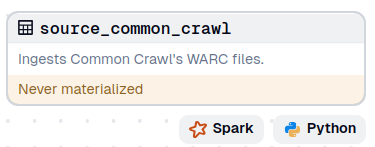
\includegraphics[width=0.4\textwidth]{figures/dagster-common-crawl-source.png}
  \caption{Common Crawl ingestion asset on Dagster's dashboard.}
  \label{fig:dagster-source-common-crawl-source}
\end{figure}

At the top of \cref{lst:dagster-source-common-crawl}, a \texttt{Configuration} class defines parameters passed to the asset, allowing for the following customizations:

\begin{itemize}
    \item \textbf{dataset\_id} allows specification of a Common Crawl dataset, with the default set to the most recent dataset.
        For instance, setting \texttt{CC-MAIN-2024-42} accesses data from October 2024, while \texttt{CC-MAIN-2024-33} refers to August 2024.
        This flexibility is crucial, as each dataset contains approximately 100~TiB of compressed data, requiring significant ingestion time, especially since new datasets are released monthly.
    \item \textbf{dataset\_subset} enables users to ingest data beyond the default \ac{warc} files, which contain only responses with status code \texttt{200}.
        For example, setting \texttt{non200responses} allows ingestion of \ac{http} responses with status codes indicating unsuccessful results—a dataset comprising around 2.5~TiB of compressed data across 90,000 files in Common Crawl.
    \item \textbf{path\_filter\_regex} specifies which of the approximately 90,000 \ac{warc} files to load from a dataset.
        For example, the regex \texttt{\textasciicircum.+-00000\textbackslash.warc\textbackslash.gz\$} restricts processing to 100 files, selecting one file per batch of 900 \ac{warc} files.
        By default, only the first \ac{warc} file is processed; a regex like \texttt{*} can be used for full dataset ingestion in production.
    \item \textbf{max\_batch\_size} adjusts the data size in each Spark job.
        While Spark jobs default to 128 MiB, we configure Spark to handle jobs up to 1 GiB to improve performance, aligning with this parameter's default.
        This setting primarily provides flexibility if smaller job sizes prove necessary.
\end{itemize}

\Cref{lst:dagster-source-common-crawl-fetch} demonstrates how Common Crawl data is fetched via its secure \ac{http} \ac{api}.
First, the available datasets are pulled from Common Crawl's index (lines 3 and 4) if no \texttt{dataset\_id} is specified.
Next, \ac{warc} file metadata for the given dataset is pulled from Common Crawl's data storage, as shown in lines 16 to 20.
The metadata is compressed with \href{https://www.gnu.org/software/gzip/}{\textit{gzip}} and must be decompressed (line 24) and decoded in \href{https://www.unicode.org/versions/latest/}{\texttt{UTF-8}} (line 25).
Finally, each \ac{warc} file is fetched in the last function, defined from lines 40 to 45.
Two Python decorators serve as helper functions in \cref{lst:dagster-source-common-crawl-fetch}:

\begin{itemize}
    \item \textbf{measure\_performance} is a custom function that helps identify performance bottlenecks by using Python's built-in time and logging functionalities, as specified in \cref{lst:dagster-utility-performance-measurement}.
    \item \textbf{retry} is the exponential backoff implementation from the \texttt{tenacity} library, enabling retries on temporary \ac{http} 503 error responses.
\end{itemize}

The main ingestion logic is outlined in \cref{lst:dagster-source-common-crawl-warc}.
The archive stream retrieved from the previously fetched \ac{warc} files via the \texttt{fastwarc} library is passed in at line 3, along with the dataset ID on line 4.
For each record within the stream, validations are performed for parsing success, content type, record type, \ac{http} status code, charset, and \ac{uri} validity.
These validations are represented by comments in the listing for brevity.
If the record passes these checks, the \ac{html} response within the record is decoded (line 19), and the sizes for both the encoded and decoded versions are measured (lines 23 and 24).
Finally, records that meet the table schema requirements are yielded\footnote{Values yielded by this function can be iterated over by calling functions. The function in \cref{lst:dagster-source-common-crawl-warc} is a Python \href{https://wiki.python.org/moin/Generators}{\textit{Generator}}.} (lines 26 to 34).

\begin{listing}[H]
\begin{minted}{python}
@measure_performance
def get_warc_records(
    records: ArchiveIterator,
    dataset_id: str
):
    for record in records:
        # ...http parsing verification...

        if record.http_content_type != "text/html":
            continue # skip non-html content like PDFs or XML files

        # ...record type, status code, charset and target uri verification...

        response_target_uri = record.headers.get("WARC-Target-URI")
        response_charset = record.http_charset
        response_payload = record.reader.read()

        try:
            response_payload_decoded = response_payload.decode(response_charset or "utf-8")
        except UnicodeDecodeError:
            # ...retry logic...

        response_payload_size_bytes = len(response_payload)
        response_payload_decoded_length = len(response_payload_decoded)

        yield {
            "dataset_id": dataset_id,
            "response_charset": response_charset,
            "response_headers_status_code": record.http_headers.status_code,
            "response_payload": response_payload_decoded,
            "response_payload_size_bytes": response_payload_size_bytes,
            "response_payload_length": response_payload_decoded_length,
            "response_target_uri": response_target_uri,
        }
\end{minted}
\caption{Extraction of Common Crawl's \ac{warc} data.}
\label{lst:dagster-source-common-crawl-warc}
\end{listing}

The records extracted from the \ac{warc} files are then accumulated until a specific batch size is reached by the function defined in \cref{lst:dagster-utility-performance-batching}.
To further enhance performance, a queue of such batches is used, allowing multiple batches to be generated in advance while they are sequentially processed in the next step.
The queuing mechanism improves performance by ensuring the immediate availability of the next item for processing.
If each batch were generated only after the preceding batch completed its processing, valuable time would be lost in generating the next item.
This queue implementation leverages Python's asynchronous \ac{io} module, as shown in \cref{lst:dagster-utility-performance-queuing}.

To complete the ingestion tooling, we configure a Spark client for writing extracted records to Iceberg tables.
\Cref{lst:dagster-utility-spark} shows a PySpark client instance, named \texttt{SparkSession}, implemented with a \textit{Singleton} pattern.
The Spark driver is configured to receive inbound traffic on port 7777, which would otherwise be randomly selected.
Specifying a port allows us to establish strict networking rules in Kubernetes, though this is unnecessary when running in Docker Compose.
Similarly, port 7878 is set for Spark's block manager, which supports data broadcasting to executors.
Most other configuration settings align with those previously discussed for Spark configurations, such as the \texttt{rest} service setup in \cref{sec:implementation-infrastructure-compute}.

The Spark client configuration also provides flexible memory reservation for the Spark driver and executors: 50~G is reserved when running on a Kubernetes cluster and 4~G when running in Docker Compose.
In this context, running on Kubernetes equates to production, and these memory values (50~G and 4~G) are chosen based on the available memory on the production and development machines.

To complete the Common Crawl ingestion, the fetched data is written to its designated Iceberg table.
\Cref{lst:dagster-source-common-crawl-write} shows a general, type-safe approach for writing to this table.
The schema defined in the initial lines ensures that a table can be created even when the initial data does not clearly allow for schema inference -- for example, when a column filled exclusively with \texttt{null} values makes it impossible to determine an appropriate type such as \texttt{string} or \texttt{integer}.

The logic for choosing between appending to or creating a table (lines 15 to 18) could be streamlined if a \texttt{createOrAppend} command were available.
Although a \texttt{MERGE INTO} \ac{sql} command exists for Iceberg, it is only accessible via the \textit{Data Source V2} \ac{api} in Spark \texttt{4}, which has not yet been released at the time of writing~\cite{Gao2023}.
The \texttt{spark\_dataframe.mergeInto("table")} function in Spark \texttt{4} would also prevent duplicate row insertions, which are currently managed manually, as shown in \cref{lst:dagster-source-common-crawl-write-deduplicated}.
\Cref{fig:analysis-pipeline-performance-driver} shows the Spark driver's query diagram for this data appending operation.
Tables with few rows, where full refreshes are feasible with each update, may alternatively use \texttt{spark\_dataframe.createOrReplace("table")}.

\begin{listing}[H]
\begin{minted}{python}
SCHEMA = StructType(
  [
    StructField("dataset_id", StringType(), False),
    StructField("response_headers_status_code", IntegerType(), False),
    # ...more fields...
  ]
)
TABLE = "raw.source_common_crawl"


def write_source(batch: list):
  is_table_existing = SparkManager.spark.catalog.tableExists(TABLE)
  dataframe = SparkManager.spark.createDataFrame(batch, SCHEMA)

  if is_table_existing:
    dataframe.writeTo(TABLE).append()
  else:
    dataframe.writeTo(TABLE).partitionedBy("dataset_id", "response_charset").create()
\end{minted}
\caption{Writing entries to a partitioned Iceberg table.}
\label{lst:dagster-source-common-crawl-write}
\end{listing}

We have now defined a complete ingestion flow into the bronze layer, as defined in \cref{sec:design-decisions-elt}.
Next, we proceed with transformations from the bronze layer to the silver and gold layers.


\subsubsection{Transformation}
\label{sec:implementation-pipeline-transformation}

With data ingested into the bronze layer, represented by the namespace \texttt{raw}, we first use dbt to transform data into the silver layer, represented by the namespace \texttt{staging}.
We then use a Dagster Python asset to combine all silver-layer tables into a \texttt{fact} table stored in the gold layer.

Python is used instead of dbt for the final transformation to showcase how a transformation leveraging a third-party Python module can be implemented, extending beyond the capabilities of \ac{sql} statements.
This Python example also illustrates the potential for bidirectional asset connections in Dagster, meaning connections can be made from Python assets to dbt models and vice-versa.

Given the distinct natures of our two transformation types, dbt code is primarily declarative, while Python code is imperative.
The following code listings will therefore primarily show configuration declarations instead of imperative code for dbt.

A basic dbt setup includes a project configuration and a profile configuration.
The project configuration allows us to define models, seeds, snapshots, variables, and general project settings, such as name and version, as well as adjust the directory paths where dbt expects to find source files.
The profile configuration defines storage connections.

Similar to \cref{sec:implementation-pipeline}, we set up a new dbt project named \texttt{transformation} with the following dependencies managed by Poetry:

\begin{itemize}
  \item \textbf{dbt-core} for dbt itself.
  \item \textbf{dbt-spark} with the \texttt{PyHive} extra to enable dbt connections to Spark via Thrift.
\end{itemize}

Our dbt project configuration, shown in \cref{lst:implementation-pipeline-transformation-dbt-project}, sets \texttt{iceberg} as the file format on lines 5 and 11 and outputs to the \texttt{staging} namespace\footnote{In dbt, a schema is equivalent to an Iceberg database and namespace.} (line 9), materialized as a view (line 8).
The straightforward transformations we perform, such as renaming columns and excluding rows where certain fields are \texttt{null}, do not require table materialization, which would largely result in duplicated data.
An additional option dbt offers is incremental materialization, which only processes new and updated data based on a specified strategy, such as \texttt{append} or \texttt{merge}.
For our basic transformations, a view is both sufficient and efficient.

Our dbt project is also configured with a seed table named \texttt{seed\_common\_crawl} in the \texttt{raw} namespace (starting from line 10).
With the configuration in \cref{lst:implementation-pipeline-transformation-dbt-project}, dbt loads a \ac{csv} file named \texttt{seed\_common\_crawl} into an identically named table within the \texttt{raw} namespace when running \texttt{dbt seed}.

\begin{listing}[H]
\begin{minted}{yaml}
name: 'transformation'
profile: 'transformation'
# ...more properties...
models:
  +file_format: iceberg
  transformation:
    staging:
      +materialized: view
      +schema: staging
seeds:
  +file_format: iceberg
  +schema: raw
  transformation:
    seed_common_crawl:
      +column_types:
        dataset_id: string
        response_headers_status_code: int
        # ...more columns...
\end{minted}
\caption{Configuration of our dbt project.}
\label{lst:implementation-pipeline-transformation-dbt-project}
\end{listing}

\Cref{lst:implementation-pipeline-transformation-dbt-model} shows the definition for the dbt model \texttt{dimension\_web\_technologies}.
This model is configured to select four columns (lines 1 to 5) from the bronze layer's \texttt{raw.source\_common\_crawl} table, renaming one of the columns (line 3) and ensuring all rows have values in two columns (line 6).
Line 6 includes a templating expression that is not part of the \ac{sql} standard; dbt replaces this with the appropriate value using Python's \href{https://jinja.palletsprojects.com/}{Jinja} templating engine.
To use a seed instead of a table as a source, one could specify \texttt{ref('seed\_web\_technologies')} on line 6.

\begin{listing}[H]
\begin{minted}{sql}
SELECT
  description,
  html AS html_regular_expressions,
  name,
  website
FROM {{ source('raw', 'source_web_technologies') }}
WHERE html IS NOT NULL AND name IS NOT NULL
\end{minted}
\caption{The dbt model \texttt{dimension\_web\_technologies}.}
\label{lst:implementation-pipeline-transformation-dbt-model}
\end{listing}

In addition to a model definition, we also define a dbt macro, shown in \cref{lst:implementation-pipeline-transformation-dbt-macro}, to demonstrate dbt's testing capabilities.
Beyond built-in checks like \texttt{not\_null} and \texttt{unique}, this custom check validates that only expected status codes have been transformed into the silver stage.
If the query in the macro returns any values, the transformation fails, printing the number of offending rows.

\begin{listing}[H]
\begin{minted}{sql}

SELECT *
FROM {{ model }}
WHERE ({{ column_name }} < 200 OR {{ column_name }} > 599)

\end{minted}
\caption{A dbt macro that checks for a reasonable \ac{http} status code.}
\label{lst:implementation-pipeline-transformation-dbt-macro}
\end{listing}

\Cref{lst:implementation-pipeline-transformation-dbt-models} now integrates all components by referencing models and sources, thus making them visible to dbt.
First, the model \texttt{dimension\_common\_crawl} defined in \cref{lst:implementation-pipeline-transformation-dbt-model} is declared.
The macro from \cref{lst:implementation-pipeline-transformation-dbt-macro} is applied as a test on the column \texttt{response\_headers\_status\_code} (line 9), alongside a \texttt{not\_null} test.

Line 5 sets a description for the column using the templating syntax familiar from the macro definition.
An example documentation definition is provided in \cref{lst:appendix-listings-dbt-doc}.
The full project documentation can be generated and served using the commands specified in \cref{lst:implementation-pipeline-transformation-dbt-docs}.
An example screenshot of dbt's comprehensive project documentation is shown in \cref{fig:appendix-guis-dbt-docs}.

To make the \texttt{raw} namespace available as a source, it is declared starting on line 12.
It is important to note that lines 19 to 21 define an asset key as metadata, which allows Dagster to link dbt models to their dependencies.
Additionally, dbt enables freshness checks on source data, as shown from line 22 onward.

\begin{listing}[H]
\begin{minted}{yaml}
models:
  - name: dimension_common_crawl
    columns:
      - name: response_headers_status_code
        description: '{{ doc("common_crawl__response_headers_status_code") }}'
        data_type: number
        data_tests:
          - not_null
          - is_between_200_and_599
    #...more columns...
  #...more models...
sources:
  - name: raw
    tables:
      - name: source_common_crawl
        columns:
          - name: response_headers_status_code
          #...more columns...
        meta:
          dagster:
            asset_key: ["source_common_crawl"]
    freshness:
      warn_after: {count: 150, period: day}
      error_after: {count: 365, period: day}
      filter: datediff('year', dataset_year, current_timestamp) < 2
    loaded_at_field: dataset_year
  #...more sources...
\end{minted}
\caption{Definition of dbt models and sources.}
\label{lst:implementation-pipeline-transformation-dbt-models}
\end{listing}

Having explored the dbt project configuration and model definitions in detail, we now move back to the root-level profile definitions, which then lead us toward Dagster.
The profiles shown in \cref{lst:implementation-pipeline-transformation-dbt-profiles} allow dbt commands executed via the command line to use a different host than when run inside a container.
Line 15 specifies the default profile, \texttt{cli}, which is used by the command line if not overridden by the respective command-line argument.

\begin{listing}[H]
\begin{minted}{yaml}
transformation:
  outputs:
    cli:
      type: spark
      method: thrift
      schema: default
      host: 127.0.0.1
      port: 10000
    internal:
      type: spark
      method: thrift
      schema: default
      host: spark-iceberg
      port: 10000
  target: cli
\end{minted}
\caption{Configuration of dbt profiles.}
\label{lst:implementation-pipeline-transformation-dbt-profiles}
\end{listing}

Dagster integrates dbt as shown in \cref{lst:implementation-pipeline-transformation-dagster-dbt}, where line 9 specifies the use of the \texttt{internal} profile instead of the default \texttt{cli} profile for \acp{rpc} initiated by Dagster.
Line 2 locates the dbt project in a directory named \texttt{transformation}.
Line 19 commands the dbt project to be built, generating a dbt manifest file that Dagster uses to learn about the dbt project's models and seeds.

\begin{listing}[H]
\begin{minted}{python}
project = DbtProject(
  project_dir=Path(__file__).joinpath("transformation").resolve(),
)

Definitions(
  resources={
    "dbt": DbtCliResource(
      project_dir=project,
      target="internal"
    ),
  },
)

@dbt_assets(manifest=project.manifest_path)
def transformation_dbt_assets(
  context: AssetExecutionContext,
  dbt: DbtCliResource,
):
  yield from dbt.cli(["build"], context=context).stream()
\end{minted}
\caption{Integration of the dbt project into Dagster.}
\label{lst:implementation-pipeline-transformation-dagster-dbt}
\end{listing}

Our dbt project is now fully integrated with Dagster and the Dagster \ac{gui} displays it as shown in \cref{fig:dagster-source-common-crawl}.
There are two new boxes with dbt tags, representing the seed declared in \cref{lst:implementation-pipeline-transformation-dbt-project} and the model definition from \cref{lst:implementation-pipeline-transformation-dbt-model}.
The silver layer's dimension asset also lists seven checks, representing the total number of tests like \texttt{is\_between\_200\_and\_599} or \texttt{not\_null} across all columns.
A gray dot is shown next to the number seven, indicating that none of the tests have been executed yet.

\begin{figure}[H]
  \centering
  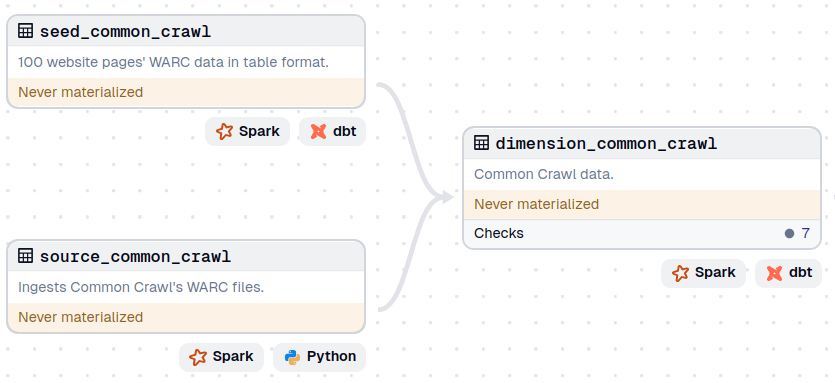
\includegraphics[width=0.75\textwidth]{figures/dagster-common-crawl.png}
  \caption{Common Crawl bronze and silver layers' assets on Dagster's dashboard.}
  \label{fig:dagster-source-common-crawl}
\end{figure}

The only remaining transformation is between the silver layer and the gold layer.
As this is a more complex transformation\footnote{Another similar transformation, not shown here for brevity, uses a third-party Python library.}, we use Python instead of dbt, as shown in \cref{lst:implementation-pipeline-transformation-fact}.

Lines 1 to 8 define a Dagster asset that depends on the dbt model \texttt{dimension\_common\_crawl}.
The complex transformation is defined as a lambda function in lines 13 to 20.
The function takes in \ac{html} code, searches for web technology usage within the \ac{html} code via \ac{regex} pattern matching, and returns a list of detected web technology names.
To use this function with Spark, it is converted into a \ac{udf} in lines 21 to 24.
The \ac{udf} is then applied to a column containing \ac{html} data (line 28), creating a new \texttt{web\_technologies} column in the existing DataFrame.
The final result is written to the \texttt{fact\_website} table in the \texttt{marts} namespace, representing the gold layer.

\begin{listing}[H]
\begin{minted}{python}
@asset(
  deps=[
      get_asset_key_for_model(
        [transformation_dbt_assets], "dimension_common_crawl"
      ),
  ],
  kinds={"python", "spark"},
)
def fact_website():
  web_technologies = SparkManager.spark.table(
    "staging.dimension_web_technologies"
  ).collect()
  get_web_technologies: Callable[[str], list[str]] = lambda html: [
      web_technology["name"]
      for web_technology in web_technologies
      if any(
          re.search(regular_expression, html)
          for regular_expression in web_technology["html_regular_expressions"]
      )
  ]
  get_udf = udf(
    get_web_technologies,
    ArrayType(StringType())
  )

  common_crawl = SparkManager.spark.table("staging.dimension_common_crawl")
  common_crawl = common_crawl.withColumn(
      "web_technologies", get_udf(common_crawl["response_payload"])
  )
  common_crawl.writeTo("marts.fact_website").createOrReplace()
\end{minted}
\caption{Transformation of staging tables into a fact table.}
\label{lst:implementation-pipeline-transformation-fact}
\end{listing}

The result, along with two additional source definitions for country codes and web technologies (omitted here for brevity), is displayed in \cref{fig:implementation-dx-dashboard}.
In that figure, parts of the overall workflow have been executed or are currently running.
All assets in the bronze layer and one dimension table have been successfully materialized.
The \texttt{dimension\_common\_crawl} asset was materialized, with one check having failed, one succeeded, and five still in progress.
The \texttt{dimension\_web\_technologies} asset shows all checks failing, indicating an issue with the dependent source table.
The gold layer's \texttt{fact\_table} asset is still in the process of materializing.

\begin{figure}[H]
  \centering
  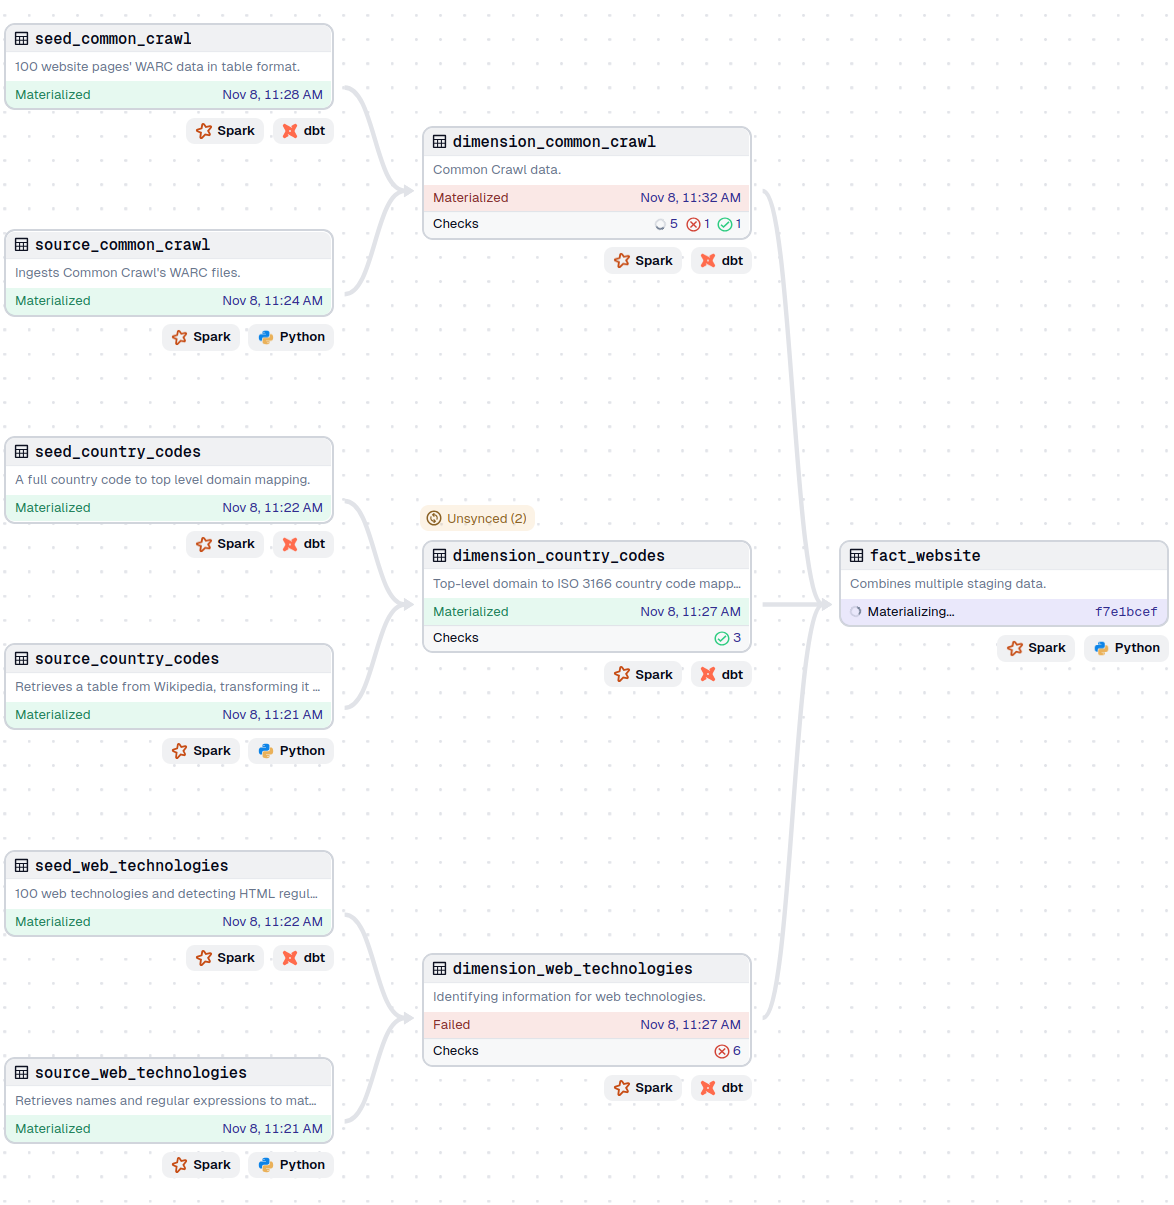
\includegraphics[width=\textwidth]{figures/dagster-white-ui-cut.png}
  \caption{Dagster dashboard of the Big Data pipeline.}
  \label{fig:implementation-dx-dashboard}
\end{figure}

A detailed examination of the country codes and web technologies assets will be left out to keep this section concise.
In brief, the country codes are fetched from a table on Wikipedia to demonstrate Pandas' basic \ac{html} extraction capabilities in \cref{lst:appendix-listings-pandas-tables}, and the data on web technologies is sourced from the \href{https://github.com/tunetheweb/wappalyzer/}{\textit{Wappalyzer}} project on GitHub.
Instead of crawling from Wikipedia, the \href{https://pypi.org/project/countrycode/}{\textit{countrycode}} Python package could be used.
Both methods are evaluated in \cref{sec:evaluation}.


\subsubsection{Visualization}
\label{sec:implementation-pipeline-visualization}

To generate graphs that visualize data from any table we create, we use \href{https://plotly.com/}{\textit{\ac{px}}}.
The implementation is straightforward: we define an example graph and then write it to a shared storage accessible by a web server.
We can then generate a link to the graph's web address and pass it as a result to Dagster's \ac{gui}.

\Cref{lst:implementation-pipeline-visualization-chart} demonstrates the generation of a choropleth map, as envisioned previously in \cref{fig:choropleth}.
First, an aggregate \ac{sql} statement is executed in a distributed manner via Spark (lines 2 to 6).
The resulting Spark DataFrame is converted into a Pandas DataFrame on line 7, as Spark DataFrames cannot be passed directly into \ac{px} functions.
The following lines configure the choropleth map.
Line 11 specifies the column that provides the country identifier in proper \href{https://www.iso.org/iso-3166-country-codes.html}{ISO 3166 alpha-3} format.
Lines 12 and 13 define the color scale used on the aggregate count, with \texttt{Viridis} chosen for optimal visibility for colorblind readers.
Lines 14 to 22 specify data displayed when hovering over countries in the map's \ac{html} version, providing detailed information that is useful for readers of the analysis in the next section.

\begin{listing}[H]
\begin{minted}{python}
def get_chart_fact_uri_choropleth():
  df_spark = SparkManager.spark.sql("""
    SELECT iso_3166_alpha3, country, COUNT(uri)
    FROM marts.fact_website
    GROUP BY iso_3166_alpha3, country
  """)
  df_pandas = df_spark.toPandas()

  graph = px.choropleth(
    df_pandas,
    locations="iso_3166_alpha3",
    color="count(uri)",
    color_continuous_scale=px.colors.sequential.Viridis,
    hover_data=["count(uri)", "iso_3166_alpha3"],
    hover_name="country",
    labels={
      "count(uri)": "Count",
      "iso_3166_alpha3": "ISO 3166-1 alpha-3 code",
    },
  )
  graph.update_traces(marker_line_color="white")
  graph.update_layout(
    title_text="Website Count by Country",
  )

  return graph
\end{minted}
\caption{Chart generation using Plotly.}
\label{lst:implementation-pipeline-visualization-chart}
\end{listing}

To separate transformations from visualizations, all graphs are generated by a new Dagster asset named \texttt{charts}.
Alternatively, each existing asset could be extended to output relevant graphs.

\Cref{lst:implementation-pipeline-visualization-charts} shows the new Dagster asset for chart generation.
Lines 7 to 9 exemplarily reference the chart's getter function, defined in the preceding \cref{lst:implementation-pipeline-visualization-chart}, keyed by a file name.
For each such combination -- many more are omitted here for brevity -- the graph is generated and written to storage in lines 11 to 13.

\begin{listing}[H]
\begin{minted}{python}
@asset(
  kinds={"python", "plotly"},
  deps=[fact_website],
)
def charts(context: AssetExecutionContext):
  web_server_directory = os.path.join(os.sep, "srv", "charts")
  charts = {
    "chart_fact_uri_choropleth": get_chart_fact_uri_choropleth, # ...
  }

  for file_name, chart_function in charts.items():
    chart = chart_function()
    chart.write_html(os.path.join(web_server_directory, file_name + ".html"))

  context.add_output_metadata(
    {
      "Charts": MetadataValue.url(
        "https://charts.big-data-pipeline.uni-kassel.dev/"
        if IS_KUBERNETES
        else "http://0.0.0.0:3001/"
      ),
    },
  )
\end{minted}
\caption{Chart output with dashboard linking.}
\label{lst:implementation-pipeline-visualization-charts}
\end{listing}

Finally, the \ac{url} to view the generated charts is added as output metadata to the Dagster asset, allowing convenient access through the Dagster workflow \ac{gui}, as shown in \cref{fig:implementation-visualization-metadata}.
The \ac{url} where the web server is available differs between development and production environments, as specified in lines 18 to 20 of \cref{lst:implementation-pipeline-visualization-charts}.

\begin{figure}[H]
  \centering
  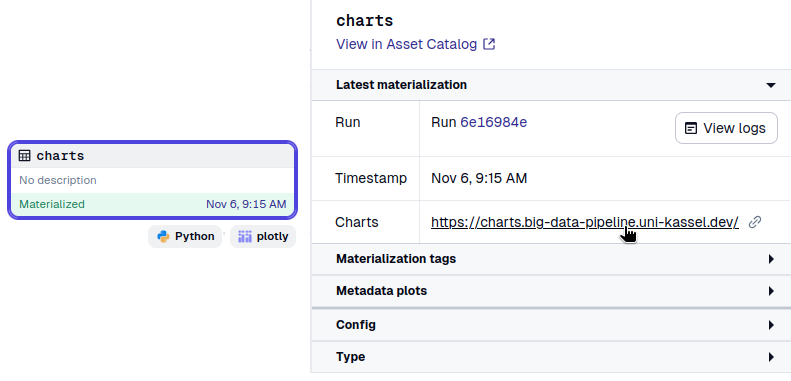
\includegraphics[width=0.85\textwidth]{figures/dagster-asset-metadata.png}
  \caption{The web server link in the \texttt{chart} asset's materialization metadata.}
  \label{fig:implementation-visualization-metadata}
\end{figure}

\subsubsection{Orchestration}
\label{sec:implementation-pipeline-orchestration}

To complete the Dagster service implementation, we define a multistage Dockerfile that allows building container images for both development and production, shown in \cref{lst:appendix-listings-dockerfile}.
This Dockerfile defines five stages for build time efficiency and \ac{dx}:

\begin{enumerate}
  \item \textbf{base-image} defines environment variables, installs \ac{os} dependencies, and sets up a rootless user, serving as the basis for stages 2 and 3.
  \item \textbf{development} builds on stage 1. It configures an entrypoint, a command, volumes, and a port to expose, all for development only. This setup allows the project to run in a container during development, ensuring a predictable environment\footnote{Refer to the open \href{https://containers.dev/}{\textit{Development Container}} specification for more on this concept.}.
  \item \textbf{prepare} also builds on stage 1, skipping stage 2. It installs Python dependencies and is intended as an incrementally extended base image for subsequent stages. For example, a \texttt{lint} stage could be added as a sibling to \texttt{build}, based on the \texttt{prepare} stage, to validate code formatting using \href{https://docs.astral.sh/ruff/}{\textit{Ruff}}.
  \item \textbf{build} builds on stage 3, copies all source code into the image, and builds the dbt project through Dagster's dbt extension.
  \item \textbf{production} builds on stage 4, installing \ac{os} dependency updates as the root user before reverting to the rootless user, and declares the command, volume, and port for production. The default command runs Dagster's webserver, but this command can be overridden in the container orchestrator's configuration to run Dagster's daemon for sensor, backfill, and scheduler support as well.
\end{enumerate}

In addition to enabling the building of development and production images, this image can serve as a substitute for a proprietary \ac{ci} pipeline.
Only minimal code needs to be written in a proprietary \ac{ci} pipeline format to initiate the Dockerfile's build process.

To build the development image, the command shown on line 1 of \cref{lst:dockerfile-build} can be executed in the working directory containing the Dockerfile.
The command on line 2 builds the final stage defined in the Dockerfile, along with all stages on which the final stage transitively depends (i.e., all stages except the \texttt{development} stage).

\begin{listing}[H]
\begin{minted}{bash}
docker build -t dargmuesli/web-kraken:dev --target development . # development
docker build . # ci
\end{minted}
\caption{Commands to build the Dockerfile.}
\label{lst:dockerfile-build}
\end{listing}

With the development image now available for our Dagster service, we can circle back to the Docker Compose infrastructure definitions in \cref{sec:implementation-infrastructure} and define a configuration for the Dagster service.
\Cref{lst:compose-dagster} shows this configuration.
On line 6, the image generated by the command on line 1 of \cref{lst:dockerfile-build} is used.
The Dagster service is also configured to start only when the Spark master and workers are available, ensuring that workflows cannot run while the Spark master or workers are still booting (lines 3 to 5).
Ports used by the Dagster container are \texttt{3000} for the main workflow \ac{gui}, \texttt{4040} for the Spark driver \ac{gui}, and \texttt{7777} for Spark's driver \ac{api} (lines 11 to 14).
Two volumes persist Dagster's workflow run data, including logs and generated charts (lines 16 to 18 and 21 to 23).
Two additional volumes, mounting a host directory into the container, enable a true Development Container experience: changes in the source code are directly accessible to Dagster without requiring a service restart (lines 19 and 20).

\begin{listing}[H]
\begin{minted}{yaml}
services:
  dagster:
    depends_on:
      - spark-iceberg
      - spark-iceberg-worker
    image: dargmuesli/web-kraken:dev
    environment:
      - AWS_ACCESS_KEY_ID=admin
      - AWS_SECRET_ACCESS_KEY=password
      - AWS_REGION=us-east-1
    ports:
      - 3000:3000
      - 4040:4040
      - 7777:7777
    restart: unless-stopped
    volumes:
      - dagster_data:/home/rootless/dagster
      - httpd_data:/srv/charts
      - ./orchestration:/srv/app
      - ./transformation:/srv/transformation
volumes:
  dagster_data: {}
  httpd_data: {}
\end{minted}
\caption{Docker Compose definition for Dagster.}
\label{lst:compose-dagster}
\end{listing}

With this, we have implemented all services for scheduling via Docker Compose.
For production, we need to define Kubernetes resources, as described in the next section.


\subsection{Deployment}
\label{sec:implementation-deployment}

The services from \cref{sec:implementation-infrastructure} and \cref{sec:implementation-pipeline-orchestration} were defined for development deployment using Docker Compose.
This section outlines the necessary modifications for production deployment using Kubernetes.

The bulk of the migration from a \texttt{docker-compose.yaml} file to Kubernetes resource definitions can be handled with Kompose, which translates each declaration individually.
However, not every declaration can or should be translated in isolation.

For example, Kubernetes' concept of \texttt{pods} allows the \texttt{dagster} container definition to be merged with the \texttt{httpd} container definition within the same pod.
This merging into a single pod is necessary, as the shared storage currently only supports the \texttt{ReadWriteOnce} access mode, which prevents mounting this volume for multiple deployments\footnote{\texttt{ReadWriteMany} is available starting with Harvester v1.4.0-rc2, paired with Rancher v2.8.8 (csi-driver 0.1.19) and v2.9.2 (csi-driver 0.2.0)~\cite{TachunLin2024}.}.
Additionally, no entrypoint script is needed for \texttt{httpd} to correct filesystem permissions for the mounted shared storage, as Kubernetes allows specification of the desired filesystem permissions directly.

To ensure a correct order of resource deployment, we define several custom resource definitions as detailed in the following enumeration.

\begin{enumerate}
  \item \texttt{minio}
  \begin{enumerate}
    \item \texttt{Secret} \textbf{minio-secrets} defines S3 secrets and MinIO's \ac{gui} credentials.
    \item \texttt{PersistentVolumeClaim} \textbf{minio-data} reserves 1~TiB of storage.
    \item \texttt{Service} \textbf{minio} makes ports \texttt{9000} and \texttt{9001} accessible.
    \item \texttt{Deployment} \textbf{minio} defines the MinIO container with dependencies on the previously defined secrets and volume.
    \item \texttt{Job} \textbf{minio-client} is the equivalent of the MinIO client definition from \cref{lst:minio-client-compose} that initializes a bucket once.
  \end{enumerate}

  \item \texttt{rest}
  \begin{enumerate}
    \item \texttt{Service} \textbf{rest} makes port \texttt{8181} accessible. It must be defined before the \texttt{Deployment} as the catalog implementation requires knowledge of the assigned address at boot, which Kubernetes makes available to containers through environment variables once a \texttt{Service} is assigned.
    \item \texttt{Deployment} \textbf{rest} defines the \texttt{rest} container and additionally sets the \texttt{REST\_PORT} environment variable to override the environment variable of the same name automatically set by Kubernetes due to the preceding \texttt{Service} definition.
  \end{enumerate}

  \item \texttt{spark-iceberg-configmap}
  \begin{enumerate}
    \item \texttt{ConfigMap} \textbf{spark-iceberg-defaults} prepares the Spark defaults for usage by both the Spark master and Spark workers.
  \end{enumerate}

  \item \texttt{spark-iceberg-master}
  \begin{enumerate}
    \item \texttt{ConfigMap} \textbf{spark-iceberg-master} adds the Spark master's entrypoint script.
    \item \texttt{Service} \textbf{spark-iceberg} makes ports \texttt{7077}, \texttt{8080}, \texttt{8888}, and \texttt{10000} accessible.
    \item \texttt{Deployment} \textbf{spark-iceberg} defines the Spark master container, mounting its entrypoint with \texttt{0744} permissions so it is executable.
  \end{enumerate}

  \item \texttt{spark-iceberg-worker}
  \begin{enumerate}
    \item \texttt{ConfigMap} \textbf{spark-iceberg-worker} adds the Spark workers' entrypoint script.
    \item \texttt{Service} \textbf{spark-iceberg-worker} makes ports \texttt{7878} and \texttt{8787} accessible.
    \item \texttt{StatefulSet} \textbf{spark-iceberg-worker} defines seventeen Spark worker containers, one less than the nodes available in the cluster, as one node should remain hosting only the Spark master\footnote{Node affinity will be evaluated in \cref{sec:evaluation}}. The \texttt{StatefulSet} also mounts its entrypoint with filesystem permissions that make it executable.
  \end{enumerate}

  \item \texttt{dagster}
  \begin{enumerate}
    \item \texttt{PersistentVolumeClaim} \textbf{dagster-data} reserves 1~GiB of storage for Dagster's status management, such as log persistence of workflow runs.
    \item \texttt{PersistentVolumeClaim} \textbf{httpd-data} reserves 1~GiB of storage for charts generated to visualize insights into the stored dataset.
    \item \texttt{Service} \textbf{dagster} makes ports \texttt{3000}, \texttt{4040}, \texttt{7777}, and \texttt{7878} accessible.
    \item \texttt{Service} \textbf{dagster-httpd} makes port \texttt{3001} accessible.
    \item \texttt{Deployment} \textbf{dagster} mounts volumes with appropriate permissions that allow writes for the \texttt{rootless} user and defines the Dagster container, along with a Dagster daemon and a web server sidecar container. The web server sidecar makes the charts accessible via the web for analysis in \cref{sec:analysis}.
  \end{enumerate}

  \item \texttt{ingress}
  \begin{enumerate}
    \item \texttt{Ingress} \textbf{ingress} makes the pipeline's Dagster dashboard available at \newline\texttt{big-data-pipeline.uni-kassel.dev}. The web server hosting the charts, the Spark driver's \ac{gui}, and MinIO's dashboard are accessible at the same address, prefixed by \texttt{charts.}, \texttt{driver.}\footnote{The driver is only available while a Spark job is running.}, or \texttt{minio.}, respectively. For all addresses, the cluster's certificate manager is configured to fetch \ac{tls} certificates from \href{https://letsencrypt.org/}{\textit{Let's Encrypt}}.
  \end{enumerate}
\end{enumerate}
